\chapter{Implementation}
The implementation of the discussed methods for solving the heat equation and for model order reduction was done in Matlab.
Matlab was chosen as the programming language because it natively features matrix multiplication which finds heavy use in the previously mentioned methods.
The second reason for this selection is that ToolBoxes already implement certain model order reduction methods, such as MORLAB \cite{benner_werner} or MOR toolbox \cite{MORT}.
The following figure \ref{fig-class-1} shows the class diagram of the implementation.
\begin{figure}[H]
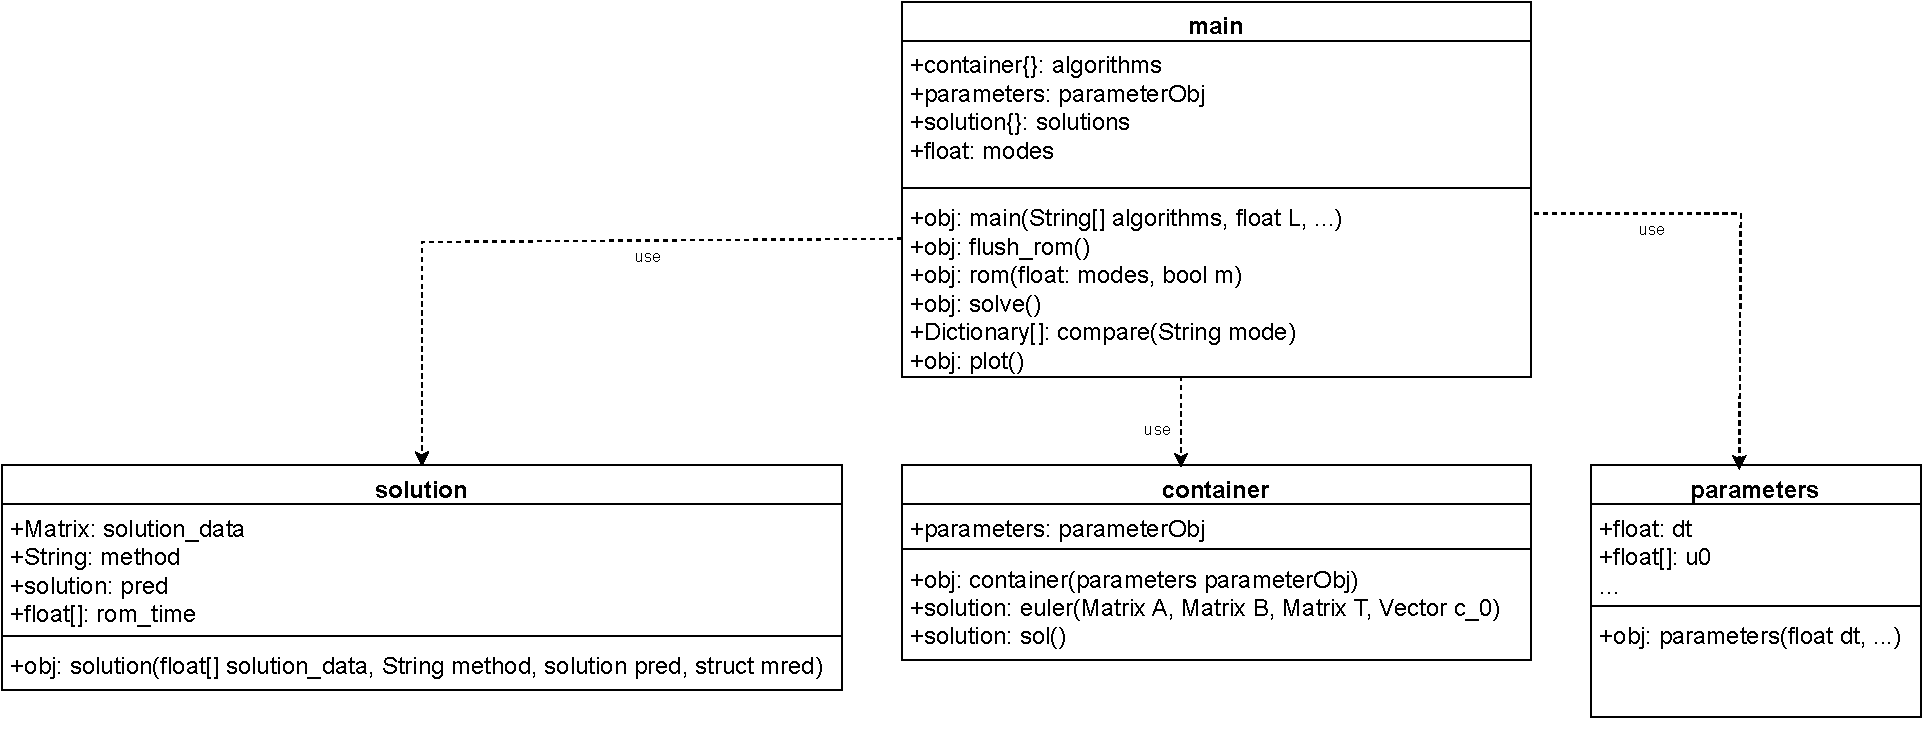
\includegraphics[width=\textwidth]{images/main}
\caption{Class diagram main}
\label{fig-class-1}
\end{figure}

\section{Class main}
The class main is responsible for generating the finite element solution, model order reduction steps, and plotting and comparing the results as well. The process can be seen in the following flow chart:
\begin{figure}[H]
\centering
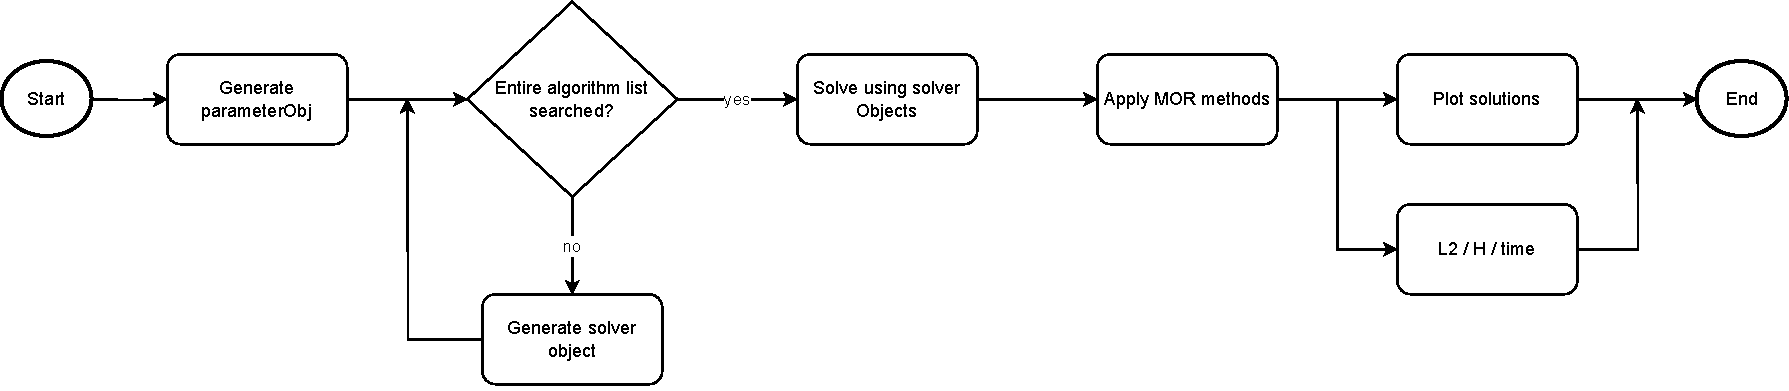
\includegraphics[ width=\textwidth]{images/main-seq}
\caption{Flow chart of main class}
\end{figure}
The first step is to generate a parameter object.
The parameter object stores all parameters to increase the transparency and robustness of the program.
The second step is to iterate the array of stated algorithms to solve the heat equation.
The options are to solve the heat equation using the finite element method section \ref{FEM} or using Fourier transform section \ref{HE}.
After all solver objects have been generated, the according solutions are computed.
After that, the MOR methods are displayed.
The final step is to display the solutions or return the \(L2\), \(H_{\infty}\) error of each ROM.
The processing time can be returned as well.

\section{Class solution}
The solution class is mainly responsible for storing solutions with some metadata.
This metadata consists of the method used to generate the stored solution, its predecessor, and computing time.
The predecessor is important to plot reduced order model solutions side by side with the original finite element solution.
The processing time is stored in an array that typically stores ten measurements.

\section{Class parameters}
The parameters class stores all parameters that have to be distributed.
They are all encapsulated within this class to make distribution and modification easier.

\section{Class container}
The container class functions like an abstract class.
It implements some methods, such as \textit{euler()}, to avoid redundancy within its child classes.
This method takes some Matrices and a vector of initial conditions and generates a solution object that stores the solution generated using an Euler scheme.
If the solution to a ROM is computed, it has to be transformed.
This step is also done here.
For this class, no objects are invoked.

\begin{algorithm}[H]
\caption{Solve a system of ODEs using Euler scheme}
\textbf{Input} \\
 \hspace*{\algorithmicindent} $A$ matrix of system \\
 \hspace*{\algorithmicindent} $B$ matrix of system \\
 \hspace*{\algorithmicindent} $T$ Coordinate transform to retrieve full state approximation of solution \\
 \hspace*{\algorithmicindent} $c_0$ Initial condition \\
 \textbf{Output} \\
 \hspace*{\algorithmicindent} solution object
\begin{algorithmic}[1]
\Procedure{euler}{}
\State $C \gets [Tc_0]$
\State $j \gets 2$
\For{$t=dt  \; \textbf{to} \; T$}
\State $c_n \gets dt A c_0 + dt B h(:, j) + c_0$
\State $c_0 \gets c_n$
\State $C(:, j) \gets T c_0$
\State $j = j+1$
\EndFor 
\State sol = solution(C, "", 0, 0)
\EndProcedure
\end{algorithmic}
\end{algorithm}
Here \(dt\), \(T\) and \(h\) are provided by the parameter object,
\(dt\) is the time step, \(T\) is the time limit to which the solution is to be computed, and \(h\) is the input to the system.
Since this method is common among all classes derived from the container class, only the solution is stored in the solution object.
The remaining fields of that object are set in the child class after the object has been returned.
Those classes derived from the container class can be seen in figure \ref{fig-class-2}.
\begin{figure}[H]
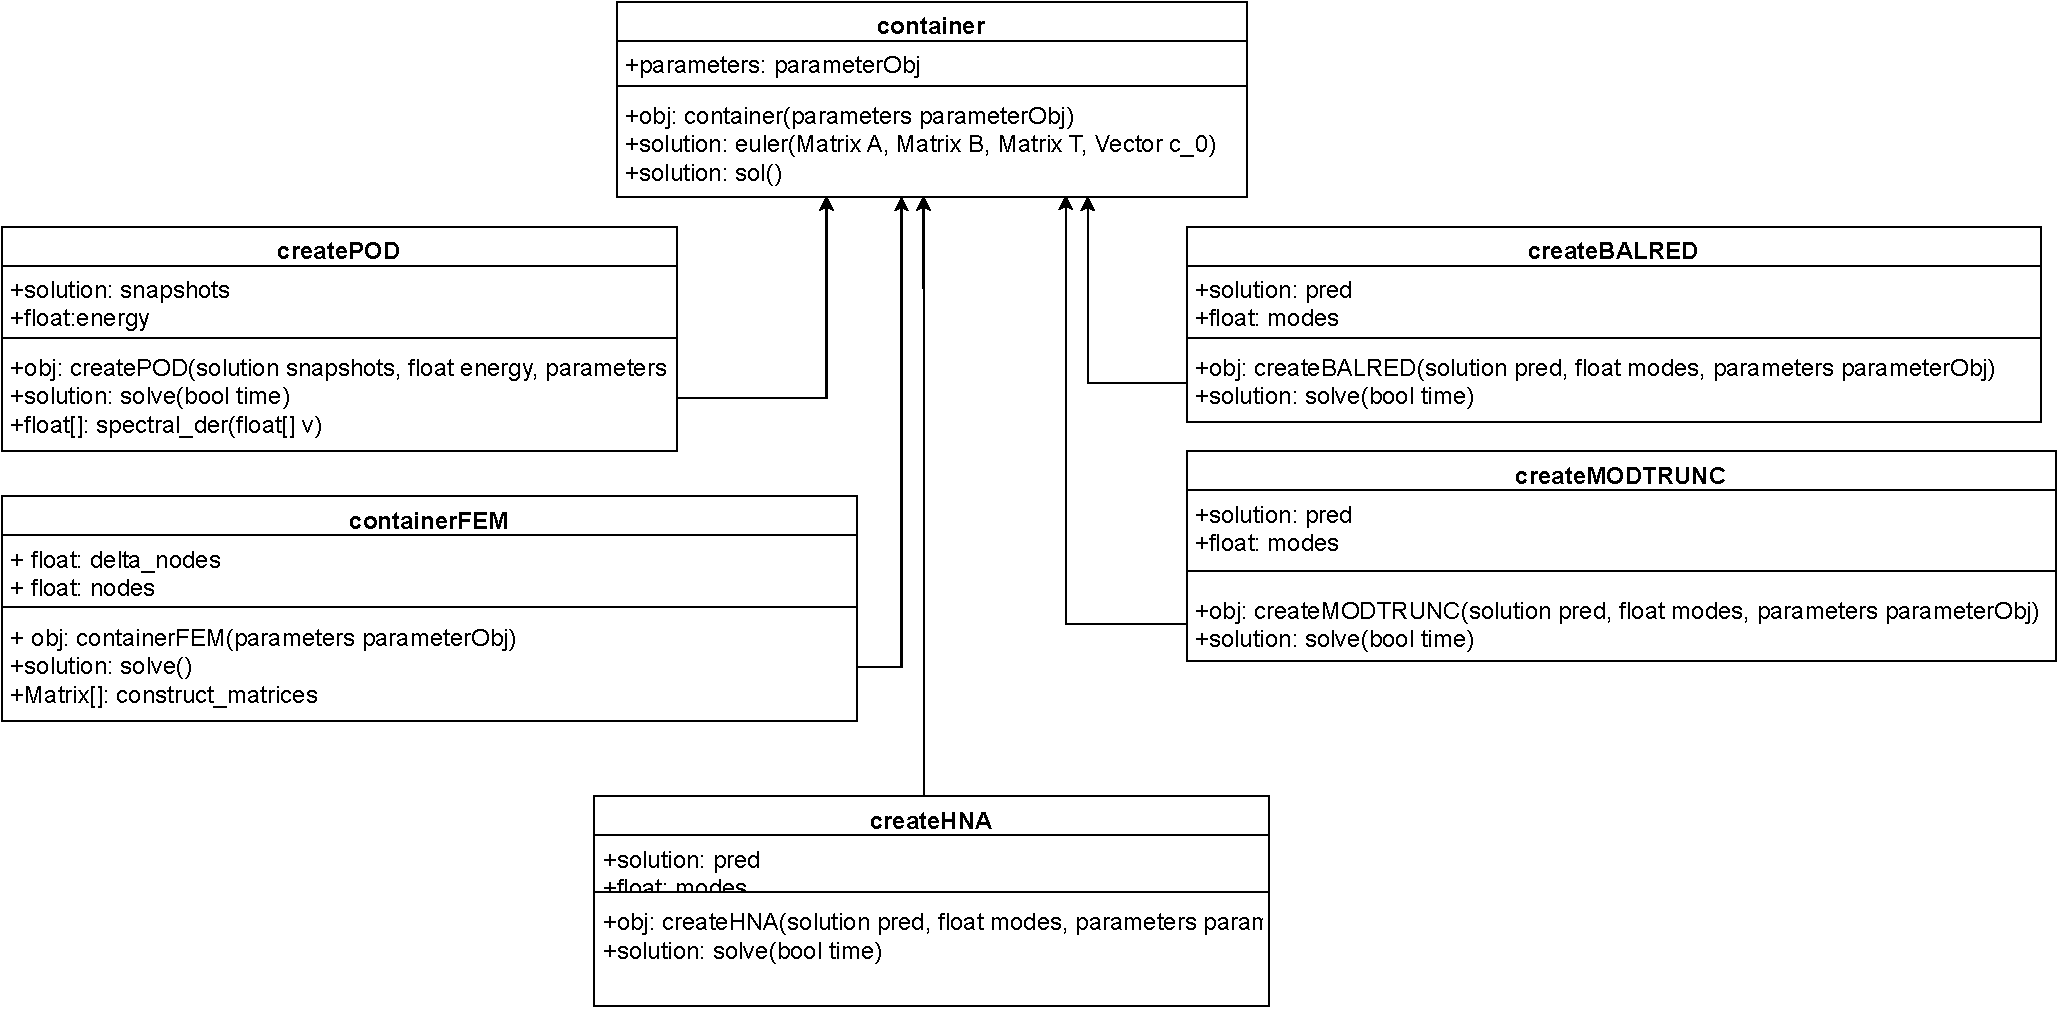
\includegraphics[width=\textwidth]{images/container}
\caption{Class diagram of MOR and FEM implementation}
\label{fig-class-2}
\end{figure}

\section{Class createBALRED, createMODTRUNC and createHNA}
Those classes are fairly simple.
MORLAB implements the actual model order reduction methods except for proper orthogonal decomposition.
Hence the according function is called and provided with the right set of parameters, and the ROM gets generated.
After that, a solution is generated using the previously described \textit{euler()} method.
For time measurements, the ROM gets generated ten times, and for each cycle, the time is stopped.
To save time, no solutions are generated in this case.

\section{Class containerFEM}
The class containerFEM generates a solution and the state space representation of the system using the finite element method.
FEM is implemented as shown in figure \ref{fig-fem-flow}.
\begin{figure}[H]
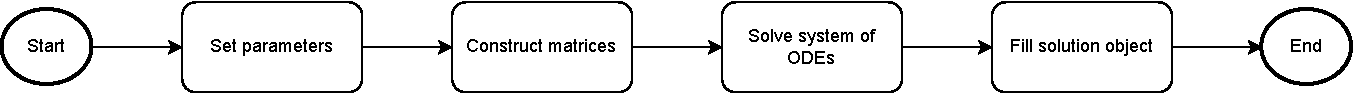
\includegraphics[ width=\textwidth]{images/seq-fem}
\caption{Flow chart for FEM class}
\label{fig-fem-flow}
\end{figure}

The first step is to set the parameters.
After that, the matrices discussed in section \ref{FEM} are being constructed.
The next step is to solve the resulting system of ODEs and pass the solution to a solution object.
\subsection{Construct Matrices}
As defined in (\ref{def-mat-a})  the matrices \(K\) and \(M\) have to be constructed.
This is done by the following method:
\begin{algorithm}[H]
\caption{Construct matrices \(K\) and \(M\)}
\textbf{Input} \\
\textbf{Output} \\
\hspace*{\algorithmicindent} [K, M]
\begin{algorithmic}[1]
\Procedure{ConstructMatrices}{}
\State $ii \gets \frac{2}{3} \Delta nodes$
\State $ij \gets \frac{1}{6} \Delta nodes$
\State $F \gets zeros(nodes, 1)$
\State $M \gets zeros(nodes)$
\For{$i=1  \; \textbf{to} \; nodes$}
\State $ K(i, i) \gets \frac{-2}{\Delta nodes}$
\State $ M(i, i) \gets ii$
\If{$i-1 > 1$}
\State $ K(i, i-1) \gets \frac{1}{\Delta nodes}$
\State $ M(i, i-1) \gets ij$
\EndIf
\If{$i+1 < nodes + 1$}
\State $ K(i, i+1) \gets \frac{1}{\Delta nodes}$
\State $ M(i, i+1) \gets ij$
\EndIf
\EndFor 
\State $\textbf{return} [K, M]$
\EndProcedure
\end{algorithmic}
\end{algorithm}

\subsection{Solve System of ODEs}
The resulting system of ODEs is solved using the implementation of the Euler scheme in the container class.
After the solution is generated, the returned solution object gets filled with the according metadata and returned.

\section{Class createPOD}
The implementation of proper orthogonal decomposition is not included in the use MORLAB package.
Therefore it is implemented in the createPOD class.
The first step is constructing the matrix \(\Phi\) as described in section \ref{chap-pod}.
This is done by computing the SVD of the provided FEM solution and truncating the resulting \(U\) matrix, such that the \(r\) most dominant modes are included.
In the following step, the transformed initial condition and the spacial derivative of \(Phi\) are computed.
The spatial derivative is computed using the spectral derivative.
In the last step, the resulting system of ODEs is solved using the implemented Euler scheme, and the resulting solution object is filled.
\begin{algorithm}[H]
\caption{Create POD}
\textbf{Input} \\
\hspace*{\algorithmicindent} $X$ Snapshot matrix \\
\hspace*{\algorithmicindent} time boolean \\
\textbf{Output} \\
\hspace*{\algorithmicindent} solution object
\begin{algorithmic}[1]
\Procedure{solve}{}
\If{time}
\For{$i=1  \; \textbf{to} \; 10$}
\State $T1 = tic$
\State [$U$, $S$, $V$] $\gets SVD(X, "econ")$
\State $\Phi = U(:, 1:r)$
\For{$i=1  \; \textbf{to} \; r$}
\State $\Phi_{xx}(:, i) \gets spectral\_der(\Phi(:, i))$
\State rom\_time(i) $\gets T1 - toc$
\EndFor
\EndFor
\State sol $\gets$ solution(NaN, "POD", $X$, NaN)
\State sol.rom\_time $\gets$ rom\_time
\EndIf
\State [$U$, $S$, $V$] $\gets SVD(X, "econ")$
\State $\Phi = U(:, 1:r)$
\For{$i=1  \; \textbf{to} \; r$}
\State $\Phi_{xx}(:, i) \gets spectral\_der(\Phi(:, i))$
\EndFor
\State $sol \gets euler(\alpha \Phi^{T} \Phi_{xx}, \Phi^{T}, \phi, \Phi^{T} u_0)$
\State rom = struct("A", $\alpha \Phi^{T} \Phi_{xx}$, "B",$\Phi^{T}$, "C", $\Phi$, "D", parameterObj.D);
\State sol.method = "Proper Orthogonal Decomposition"
\State sol.pred = $X$, sol.reduced\_model = rom
\EndProcedure
\end{algorithmic}
\end{algorithm}
From lines three to fifteen, there is some redundancy.
This section is meant to measure the processing time of POD without generating a solution.
The time measurements are stored in a solution object.
The spectral derivative is implemented in the following way.
\begin{algorithm}[H]
\caption{Compute spectral derivative}
\textbf{Input} \\
\hspace*{\algorithmicindent} $v$ Vector
\textbf{Output} \\
\hspace*{\algorithmicindent} $v'$ Derivative of $v$
\begin{algorithmic}[1]
\Procedure{spectral\_der()}{}
\State $v' \gets -k^{2}$ fft($v$)
\EndProcedure
\end{algorithmic}
\end{algorithm}
Here k are the wave numbers, and all multiplication is element-wise multiplication.

\section{Measurements}
In the next chapter, some measurements are taken to gain information about the performance and error of each method.
Therefore three sets of measurements are taken.
The first two are the \(L2\), and \(H_{\infty}\) errors of the results, and the last one is the processing time.
Further details are in the according chapter.
\subsection{L2 error}
The \(L2\) error gets determined in the \textit{compare()} method in the main class.
It gets computed in the following way.
\begin{gather}
E2 = ||S - S'||_{F}
\end{gather}
Here \(S\) is the solution of the ROM, and \(S'\) is the original FEM solution.

\subsection{$H_{\infty}$ error}
The \(H_{\infty}\) error also gets determined in the \textit{compare()} method in the main class.
\begin{gather}
H = ||S - S'||_{H_{\infty}}
\end{gather}
Here \(S\) is the transfer function of the ROM, and \(S'\) is the transfer function of the original FEM system.
\subsection{Processing time}
As already mentioned, the processing time gets determined in the according container class.
It gets passed through the \textit{compare()} method in the main class.







